\chapter{Validación de imaxes}
\minitoc
\clearpage

\section{Introdución}

Un aspecto moi a ter en conta no tratamento con contedores é a súa portabilidade, podéndoos transportar entre diferentes sistemas. Esta característica ten serias implicacións de seguridade, xa que é vital preservar e comprobar que os datos atopados no interior da imaxe non resulten alterados por unha terceira persoa. Así, ao transferir datos entre sistemas en rede e tratar cun medio non fiábel, como o é a Internet, é esencial garantir aspectos como autenticación (o creador do contedor é quen di ser), integridade (a imaxe non se viu modificada durante a transmisión) e non repudio (o creador da imaxe non pode negar que é el). Referirémonos a esta serie de aspectos como a validación das imaxes.

\section{Docker}
\label{dockerContentTruste}

Para garantir a validación de imaxes, Docker provén da ferramenta Docker Content Trust. Dita ferramenta permite a emprega de firmas dixitais, permitindo unha verificación da integridade no lado do cliente e o coñecemento do autor de etiquetas específicas dunha imaxe. Non obstante, esta utilidade non está activada por defecto, polo que o entorno debe ser configurado para isto.

\begin{lstlisting}[,caption={Activación do Docker Content Trust}]
export DOCKER_CONTENT_TRUST=1
\end{lstlisting}

As firmas dixitais son realizadas sobre as etiquetas, polo que é posíbel que existan etiquetas firmadas dunha imaxe e outras que non, sendo elección do autor se firmar unha etiqueta específica ou non. De cara ao usuario, este só poderá traballar con imaxes que estean firmadas, quedando inhabilitadas todas aquelas imaxes ou etiquetas que non o estivesen.\\

Para este control existen unha serie de chaves, que son creadas cando se invoca por primeira vez unha operación deste sistema de aseguranza da integridade. Este conxunto de chaves está conformado por:

\begin{itemize}
    \item Unha chave \textit{offline} que é a raíz do contido fiábel para unha etiqueta dunha imaxe.
    \item As chaves das etiquetas.
    \item Chaves mantidas por un servidor, como a chave do \textit{timestamp}\end{itemize}
    
A relación entre estes diferentes tipos de chaves é a seguinte: a chave \textit{offline} é empregada para crear as chaves adicadas ás etiquetas. Dita chave \textit{offline} pertence a unha persoa ou organización, e permanece en todo momento no lado do cliente, polo que debe ser almacenada nun lugar seguro e a ser posíbel, con copias de seguridade. As chaves adicadas ás etiquetas están asociadas cunha imaxe dun repositorio, sendo os creadores de dita chave os que poden realizar accións de \textit{push} e \textit{pull} sobre calquera etiqueta (\textit{tag}) do repositorio. Ao igual que a chave \textit{offline}, tamén residen no lado do cliente. A chave asociada ao \textit{timestamp} está asociada cunha imaxe dun repositorio, mais neste caso é o servidor de Docker o seu encargado, polo que reside no lado do servidor \cite{docker-content-trust}. Esta explicación pode ser apreciada na figura \ref{trust_components}. 

\begin{figure}
\centerline{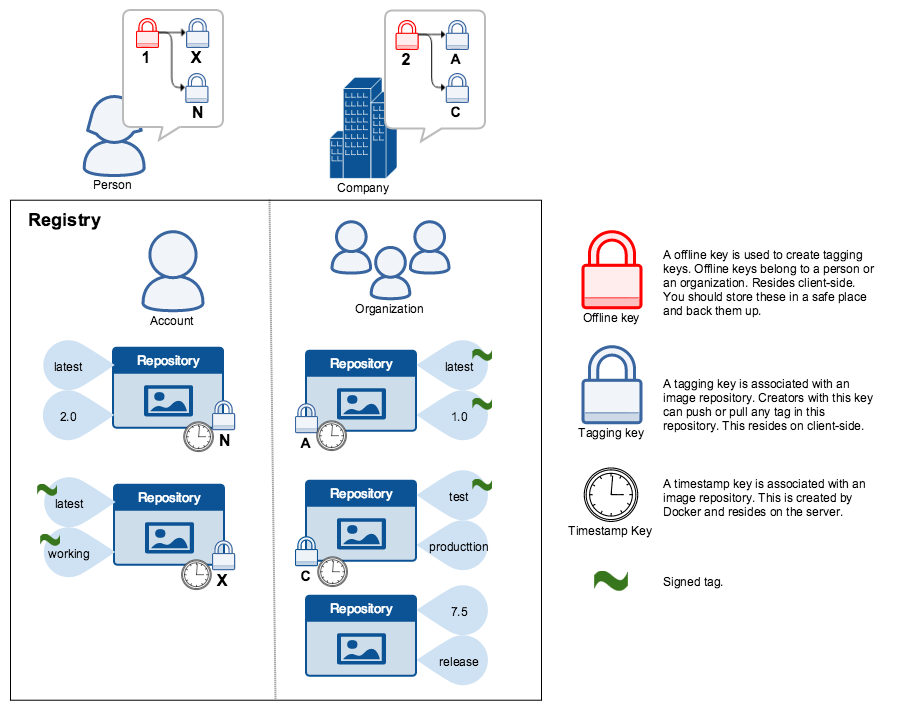
\includegraphics[width=15cm]{figuras/trust_components.png}}
\caption{Relación entre as chaves do Docker Content Trust}
\small
\centerline{Fonte: \url{https://docs.docker.com/engine/security/trust/content_trust/}}
\label{trust_components}
\end{figure}

\section{Singularity}

A validación das imaxes en Singularity é realizada mediante a integración de \textit{hashing} \gls{SHA}-256. Singularity prové un método de validación dos contedores que permite asegurar que a imaxe dun contedor que está a ser distribuído non foi alterada. Despois do proceso de \textit{bootstraping}, o \textit{hash} \gls{SHA}-256 é xerado e amosado ao usuario. Cando a imaxe é corrida máis adiante empregando a opción {\it --hash}, o seu \textit{hash} é rexenerado e amosado ao usuario.\\

O mecanismo non é tan complexo como o existente na tecnoloxía de Docker, pero segundo avisos do equipo de desenvolvemento de Singularity, a versión 3 desta tecnoloxía incluirá diversas melloras no referente a este tema \cite{SingularityLabNotes} (versión actual: 2.5.1). Por exemplo, un mecanismo similar ao de Docker no que só se poderán empregar contedores asinados, ou sistema de montaxe de contedores que permita garantir a orixe dos contedores no que poderiamos escoller só permitir executar contedores creados en certos sitios de confianza. \cite{SingularityRemoteBuild}

\section{Udocker}

Udocker non posúe ningún mecanismo propio de validación, polo que de querer aplicar un proceso de validación empregando Udocker debemos depender do Docker Content Trust explicado na sección \ref{dockerContentTruste}. Neste caso, sería preciso ter a tecnoloxía Docker instalada no sistema.
